\documentclass{beamer}

\mode<presentation>{
  \usetheme{Warsaw}
  %\usetheme{Montpellier}
  %\usetheme{PaloAlto}
  \setbeamercovered{transparent}
}

\usepackage[english,french]{babel}
\usepackage[latin1]{inputenc}
\usepackage[T1]{fontenc}
\usepackage{subfigure}
\usepackage{times}
\usepackage[french]{varioref}
\usepackage{algorithm}
\usepackage{algorithmic}
\usepackage{caption} 
%\usepackage{movie15}


%%%%%%%%%%%%%%%%%%%%%%%%%%%%%%%%%%%%%%%%%%%%%%%%%%%%%%%%%%%%
\title{Projet Tuteur� : BCI}
\subtitle{Interface Cerveau-Machine pour d�tection des diff�rents �tats d'une personne.}

\author{Nizar ABAK-KALI, Alexis ZURAWSKA}

\institute{
  PARIS VIII Saint-Denis \\
  nizarabakkali93@gmail.com,  
  zurawska.alexis@yahoo.com
  }

\date{\today}
 

\pgfdeclareimage[height=0.8cm]{le-logo}{paris8}
\logo{\pgfuseimage{le-logo}}

\AtBeginSection[]{
 \begin{frame}<beamer>{PLAN DE LA PRESENTATION}
   \tableofcontents[currentsection]
\end{frame}
}

%%%%%%%%%%%%%%%%%%%%%%%%%%%%%%%%%%%%%%%%%%%%%%%%%%%%%%%%%%%%
\begin{document}

\begin{frame}
  \titlepage
\end{frame}

\begin{frame}{PLAN DE LA PRESENTATION}
  \tableofcontents
\end{frame}

%%%%%%%%%%%%%%%%%%%%%%%%%%%%%%%%%%%%%%%%%%%%%%%%%%%%%%%%%%%%
\section{Introduction}

%%%%%%%%%%%%%ETAT DE L'ART
\begin{frame}  
  \begin{exampleblock}{Pr�sentation du Projet}
        D�tection automatique d'�tats d'un patient � partir de son signal EEG. 
        Classification des �tats et prise de decision fait par un r�seaux de neurones.\\
        Example d'�tat que l'on veut d�t�cter sur un patient atteint d'Alzheimer:
        \begin{itemize}
            \item la lecture 
            \item l'�criture
            \item l'attention sur un film
            \item la discussion
            \item le repos 
        \end{itemize}
    \end{exampleblock}
\end{frame}

%%%%%%%%%%%%%CONCEPTS
\section{Concepts}

\begin{frame}
Quelques explications sur les concepts �tudi�s et utilis�s.
  \begin{exampleblock}{EEG: �lectroenc�phalographie�}
      \begin{figure}[h]
               \centering
               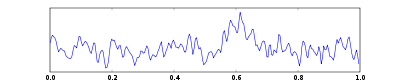
\includegraphics[scale=0.5]{eeg_1s_signal.png} 
              \captionof{figure}{ci-dessus une seconde de signal EEG}     
      \end{figure}
      \end{exampleblock}
      \begin{exampleblock}{BCI: Brain Computer Interface}
      \begin{figure}[h]
               \centering
               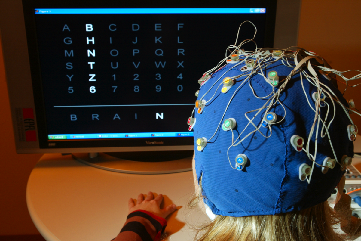
\includegraphics[scale=0.4]{bci3.png} 
              \captionof{figure}{ci dessus un BCI}
      \end{figure}  
      BCI : Brain Computer Interface
  \end{exampleblock}
\end{frame}

\begin{frame}  
  Quelques explications sur les concepts �tudi�s et utilis�s
        \begin{exampleblock}{SSVEP}        
          \begin{figure}[h]
               \centering
               %\includemovie{1cm}{1cm}{ssvep.gif}[inline=false]
              \captionof{figure}{ci-dessus une utilisation du SSVEP}     
          \end{figure}
        \end{exampleblock}
\end{frame}

\begin{frame}  
  Quelques explications sur les concepts �tudi�s et utilis�s
  \begin{exampleblock}{P300}
   \begin{figure}[h]
      \centering
     % \includemovie{1cm}{1cm}{p300.gif}[inline=false]
      \captionof{figure}{ci-dessus une utilisation du P300}     
   \end{figure}
        
\end{frame}


%%%%%%%%%%%%%%%Problematique rencontre
\begin{frame}
  \begin{alertblock}{Probl�matique rencontre}
    \begin{itemize}
    \item Comment classer les signaux r�cup�r�s ?
    \item Quels crit�res/caract�ristiques doit-on prendre en compte pour la classification ?
    \item Comment rendre notre syst�me plus performant?
    \end{itemize}
  \end{alertblock}
\end{frame}

%%%%%%%%%%%%%%%%%%%%%%%%%%%%%%%%%%%%%%%%%%%%%%%%%%%%%%%%%%%%
\section{Outils Utilises}
\begin{frame}
  \begin{exampleblock}{Outils}
   \begin{itemize}
    \item Langage : Java 
    \item IDE : IntelliJ
    \item Librairie JFreeCharts : G�n�ration de Graphiques
    \item Github 
    \item LaTex
    \item OpenOffice draw pour les sch�mas
    \item argoUML pour le diagramme de classes 
    \end{itemize}
\end{exampleblock}
\end{frame}

%%%%%%%%%%%%%%%%%%%%%%%%%%%%%%%%%%%%%%%%%%%%%%%%%%%%%%%%%%%
\section{Avancement}
\begin{frame}
  \begin{exampleblock}{Ce qui a �t� fait}
   \begin{itemize}
    \item Mise en place du d�p�t GitHub avec toutes les sources et certains documents et liens utiles
    \item D�veloppement des fonctions math�matiques
    \item D�veloppement de la classe permettant de r�cup�rer la base de donn�es pour la stocker en m�moire dans un tableau. 
    \end{itemize}
\end{exampleblock}
\end{frame}

\begin{frame}
  \begin{exampleblock}{Ce qu'il reste a faire}
   \begin{itemize}
    \item L'extraction des caract�ristiques 
    \item D�veloppement du Classifieur
    \end{itemize}
\end{exampleblock}
\end{frame}

%%%%%%%%%%%%%%%%%%%%%%%%%%%%%%%%%%%%%%%%%%%%%%%%%%%%%%%%%%%%
\begin{frame}
  \titlepage
\end{frame}
%%%%%%%%%%%%%%%%%%%%%%%%%%%%%%%%%%%%%%%%%%%%%%%%%%%%%%%%%%%%
\end{document}


